\documentclass[journal]{IEEEtran}
% IEEE Transactions on Industrial Informatics -- anonymous regular-paper draft
% Compile: latexmk -pdf main.tex
\usepackage{amsmath,amssymb,amsfonts}
\usepackage{algpseudocode}
% Local XeTeX/Tectonic builds: route IEEEtran's ptm (Times) family requests to
% the legacy Times Type1 faces so metrics match the pdfLaTeX reference build;
% the latexmk -pdf (pdfLaTeX) path is unaffected.
\usepackage{iftex}
\ifxetex
  \DeclareFontFamily{TU}{ptm}{}
  \DeclareFontShape{TU}{ptm}{m}{n}{<->ptmr8t}{}
  \DeclareFontShape{TU}{ptm}{b}{n}{<->ptmb8t}{}
  \DeclareFontShape{TU}{ptm}{m}{it}{<->ptmri8t}{}
  \DeclareFontShape{TU}{ptm}{b}{it}{<->ptmbi8t}{}
  \DeclareFontShape{TU}{ptm}{m}{sl}{<->ptmro8t}{}
  \DeclareFontShape{TU}{ptm}{m}{sc}{<->ptmr8t}{}
\fi
\usepackage{graphicx}
\usepackage{booktabs}
\usepackage{tabularx}
\usepackage{array}
\usepackage[table]{xcolor}
\usepackage{stfloats}
\usepackage{placeins}
\usepackage{url}
% Allow line breaks at any character inside URLs/DOIs so long reference links
% do not leave ragged gaps at column edges (IEEE reference layout).
\usepackage{xurl}
\usepackage{etoolbox}
\urlstyle{same}
% Cross-references and citations. The cite package renders IEEE-style citation
% groups ([14]--[16], [20], [21]) with hyperref support.
\usepackage{cite}
\usepackage[colorlinks=true,linkcolor=black,citecolor=black,urlcolor=black]{hyperref}
\hypersetup{bookmarksnumbered=true,
  pdftitle={A Configuration-Driven Runtime for Integrating Industrial Agents With Online Data Acquisition and Governed Setpoint Operations},
  pdfauthor={},
  pdfsubject={IEEE Transactions on Industrial Informatics},
  pdfkeywords={industrial agents, online data acquisition, agent-mediated control, governed setpoint control, industrial communication}}

% Float placement only; IEEEtran margins and body type remain unchanged.
\setcounter{topnumber}{4}
\setcounter{bottomnumber}{3}
\setcounter{totalnumber}{7}
\setcounter{dbltopnumber}{1}
\renewcommand{\topfraction}{0.95}
\renewcommand{\bottomfraction}{0.80}
\renewcommand{\textfraction}{0.03}
\renewcommand{\floatpagefraction}{0.72}
\renewcommand{\dbltopfraction}{0.95}
\renewcommand{\dblfloatpagefraction}{0.72}

% Tight but conventional float separation; body type and margins are unchanged.
\setlength{\textfloatsep}{8pt plus 2pt minus 3pt}
\setlength{\dbltextfloatsep}{8pt plus 2pt minus 3pt}
\setlength{\intextsep}{7pt plus 2pt minus 3pt}
\setlength{\abovecaptionskip}{3pt plus 1pt minus 1pt}
\setlength{\belowcaptionskip}{2pt plus 1pt minus 1pt}

\newcommand{\system}{the platform}

\begin{document}
\bstctlcite{IEEEbstctl}

\title{A Configuration-Driven Runtime for Integrating Industrial Agents With Online Data Acquisition and Governed Setpoint Operations}

\author{}
\markboth{IEEE Transactions on Industrial Informatics, Submitted Manuscript}{Governed Setpoint Operations}

\maketitle

\begin{abstract}
An industrial agent can use online process measurements to propose a setpoint change, but neither read access nor a plausible proposal grants write authority. We present a configuration-driven runtime that binds line, product, recipe, and run context to separate acquisition and control mappings, protocol drivers, and write limits. The design routes task-mediated and direct calls through a common authorization boundary. Handlers check write limits and revalidate proposals when approval is required. The runtime distinguishes command outcomes, setpoint readbacks, and subsequent process measurements. At 55 writable endpoints in four simulated scenes spanning five protocol families, direct probes received the expected acceptance response for all 220 admissible requests and the expected rejection for all 219 collected structural violations. All 216 available simulator readbacks matched the requested values. In a mock-driver fixture, requests outside the configured window were rejected with the window check enabled and accepted when it was removed. Neither test used a language-model agent. In a selected simulator batch with no documented selection rule, a scripted policy had lower integrated absolute error than a no-write condition in all nine valid blocks. Three language-model episodes were canceled without reaching the target band. The tests support conformance of the exercised write paths to their configured rules; they do not establish autonomous closed-loop control, end-to-end agent-to-device traceability, or physical-plant performance.
\end{abstract}

\begin{IEEEkeywords}
Industrial agents, online data acquisition, agent-mediated control, governed setpoint writing, industrial communication
\end{IEEEkeywords}

\IEEEpeerreviewmaketitle

\section{Introduction}
\IEEEPARstart{O}{n} a cast-film line, an agent may read film thickness, compare it with the production target, and propose changing line speed. The thickness measurement and speed setpoint are distinct signals, even if both use Message Queuing Telemetry Transport (MQTT). A runtime that executes such a proposal must resolve it to the correct production context and control node, then decide whether the caller is authorized and the value is admissible. After dispatch, a command receipt is not a setpoint readback, and neither is evidence that film thickness reached its target (Fig.~\ref{fig:control-path}).

Prior work addresses service supervision and skill-based manufacturing~\cite{biskupovic2025supervision,koehle2026llmdriven}, plant-facing semantic grounding and verification~\cite{graul2026aas,schall2026safe}, and multi-agent fault recovery~\cite{vyas2026detection}. We ask how a runtime can connect online acquisition and objective-driven proposals to governed writes without making either protocol access or a task's context a source of write authority. The research contribution is the operation contract that connects these stages, not a new control law or reasoning algorithm.

The runtime separates acquisition from control mappings and read access from write authority. Task-mediated and direct calls share a dispatcher. The write routes recheck approved proposals before dispatch and record command outcomes, readbacks, and later observations separately. The evaluation focuses on the write boundary; it does not establish parity between the two entry paths.

The contributions are:
\begin{enumerate}
  \item A production-scene model that binds operating context, objectives, and limits to direction-specific signal mappings and registered drivers. (Section~III.)
  \item A typed operation path that separates dispatch authorization from value admission and applies approval, revalidation, and evidence recording according to the write route. (Sections~III--V.)
  \item Direct-interface probes and fixtures that assess selected mappings and write rules in simulation, plus exploratory observations from scripted and language-model-driven runs. The tests do not establish parity between task and direct entry paths. (Section~VI.)
\end{enumerate}

\begin{figure}[!b]
\centering
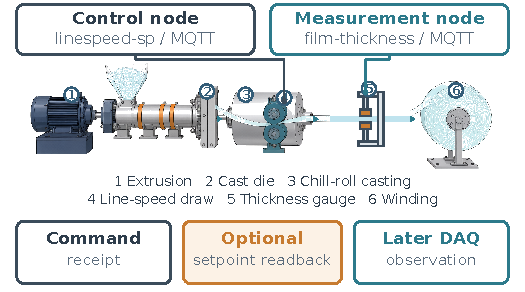
\includegraphics[width=0.98\columnwidth]{resources/fig1-vectorized-20261109.pdf}
\caption{In the cast-film example, the speed setpoint (\texttt{linespeed-sp}) and film-thickness measurement use MQTT but map to distinct nodes. A write produces a receipt and an optional setpoint readback; later film-thickness measurements are separate data-acquisition (DAQ) observations.}
\label{fig:control-path}
\end{figure}



\section{Related Work}
\label{sec:related}
Table~\ref{tab:related-comparison} summarizes the selected systems discussed below. Their different tasks, interfaces, and evaluation settings allow a qualitative comparison, not a ranking or head-to-head benchmark.

\begin{table*}[!t]
\centering
\caption{Representative related work and the scope of its reported evaluation. The studies address different tasks and are not a common benchmark. OPC UA: Open Platform Communications Unified Architecture; PLC: programmable logic controller.}
\label{tab:related-comparison}
\footnotesize
\setlength{\tabcolsep}{5pt}
\begin{tabularx}{\textwidth}{@{}>{\raggedright\arraybackslash}p{0.16\textwidth}>{\raggedright\arraybackslash}p{0.40\textwidth}X@{}}
\toprule
Study & Main focus & Reported setting \\
\midrule
Biskupovic et al.~\cite{biskupovic2025supervision} & Agent-based industrial service selection and reselection & Service adaptability and performance in an industrial cyber--physical system \\
K\"{o}hle et al.~\cite{koehle2026llmdriven} & Module-specific agents and skill-based manufacturing & Nine simulated production challenges \\
Graul et al.~\cite{graul2026aas} & Grounded proposals, documented authorization, and proposed PLC-side checks & Two proof-of-concept scenarios using a simulated OPC UA server \\
Schall~\cite{schall2026safe} & Process-diagram, supervisory control and data acquisition (SCADA), and procedure-grounded verification & Five simulated scenarios and proposal evaluation \\
Vyas et al.~\cite{vyas2026detection} & Multi-agent fault-recovery planning with a process-plant twin & Simulated mixing and stirred-tank reactor studies \\
This work & Scene-bound signal mappings, shared dispatch, and route-specific governance & Simulator and mock-driver probes, scripted policy runs, and exploratory agent-driven episodes \\
\bottomrule
\end{tabularx}
\end{table*}

\subsection{Industrial Agents and Plant Integration}
Biskupovic et al. study online service selection and reselection in industrial cyber--physical systems~\cite{biskupovic2025supervision}. Xia et al. present a digital-twin-connected automation architecture and control generation~\cite{xia2025architecture,xia2025control}; other work generates programmable logic controller (PLC) programs~\cite{liu2026agents4plc}. In related control research, human instructions have also been incorporated into model-predictive control~\cite{wu2025instructmpc}.

Li et al. use structured instructions, retrieval, and iterative verification to generate and check finite-element scripts for Abaqus; that study evaluates engineering-artifact generation rather than runtime authority over process writes~\cite{li2026modsolagent}. Other studies examine large language model (LLM) agents, manufacturing skills, and natural-language machine interaction~\cite{koehle2026llmdriven,lim2025llmenabled,zhao2026shopfloor,hofmann2025nlc}. Vyas et al. combine multi-agent fault-recovery planning and plant-knowledge retrieval with Digital Process Plant Twin models of mixing and continuous stirred-tank reactors (CSTRs)~\cite{vyas2026detection}.

These studies address agent organization, generated actions, or task execution; the present study introduces no agent policy or control law but examines the runtime boundary that carries production context and direction-specific signal mappings into an operation and applies the required checks before dispatch.

\subsection{Industrial Interfaces and Semantic Commissioning}
Agent-facing interface work includes Model Context Protocol (MCP) access to manufacturing resources~\cite{silva2025mcpmanufacturing}, semantic recipes built from Open Platform Communications Unified Architecture (OPC UA) skills~\cite{koehle2025semanticrecipes}, industrial-protocol adapters~\cite{xavier2026industriConnect}, and tools for binding manufacturing data to a cognitive digital twin~\cite{liu2026semanticcommissioning}. These systems address capability discovery, protocol access, or commissioning. Here, configuration binds known protocol drivers to scene-specific read and write nodes, and a named operation resolves those bindings through a runtime path that checks authority and write limits; neither MCP nor a semantic node name is an authorization mechanism.

\subsection{Governed Operations and Verification}
Prior work also examines plant-facing verification. Graul et al. propose grounding plans in the Asset Administration Shell, with documented human authorization and PLC-side validation of OPC UA Methods~\cite{graul2026aas}. Schall verifies proposals against piping and instrumentation diagrams, SCADA data, and standard operating procedures; Lin and Chen describe a policy-governed sensor--manufacturing execution system (MES)--enterprise resource planning (ERP) digital thread~\cite{schall2026safe,lin2026agentic}. PLCBench evaluates autonomous agents against commercial PLCs with hardware-in-the-loop process simulation~\cite{zhou2026plcbench}. These studies echo long-standing authorization and safety concerns. Our implementation asks how configured signal bindings, route-specific checks, shared dispatch, and separate command and process records operate together at the write boundary. The contribution is system integration; the studies use different settings, and none establishes comparative safety.

\subsection{Production Context and Outcome Evidence}
MCP standardizes tool discovery and invocation~\cite{mcp2026}; it does not assign plant write authority. ISA-88 and ISA-95 supply recipe and production-operation concepts~\cite{isa88_2010,isa95_2025}. Run-to-run control motivates using observations in subsequent decisions, and human--automation research motivates separating proposal and approval~\cite{moyne2001r2r,parasuraman2000model}. The distinction here is the responsibility of the runtime: resolve an intent to the active scene and its direction-specific mappings, decide whether the operation may proceed, and return evidence without conflating command, readback, and process observation. The comparison is about where these responsibilities sit, not whether another system could implement them.

\section{System Design}
\label{sec:design}
The runtime exposes named operations through two paths (Fig.~\ref{fig:arch}). In a task, a registered agent harness is the adapter that exposes scoped tools for data acquisition (DAQ) and intent submission. An agent uses observations and the task objective to analyze what to propose; it does not decide whether a write is authorized. Direct representational state transfer (REST) or stdio MCP calls invoke operations without a task. The architecture routes both entries through one dispatcher; Section~\ref{sec:eval} tests selected direct calls, not equivalent behavior across both entries.

\begin{figure*}[!t]
\centering
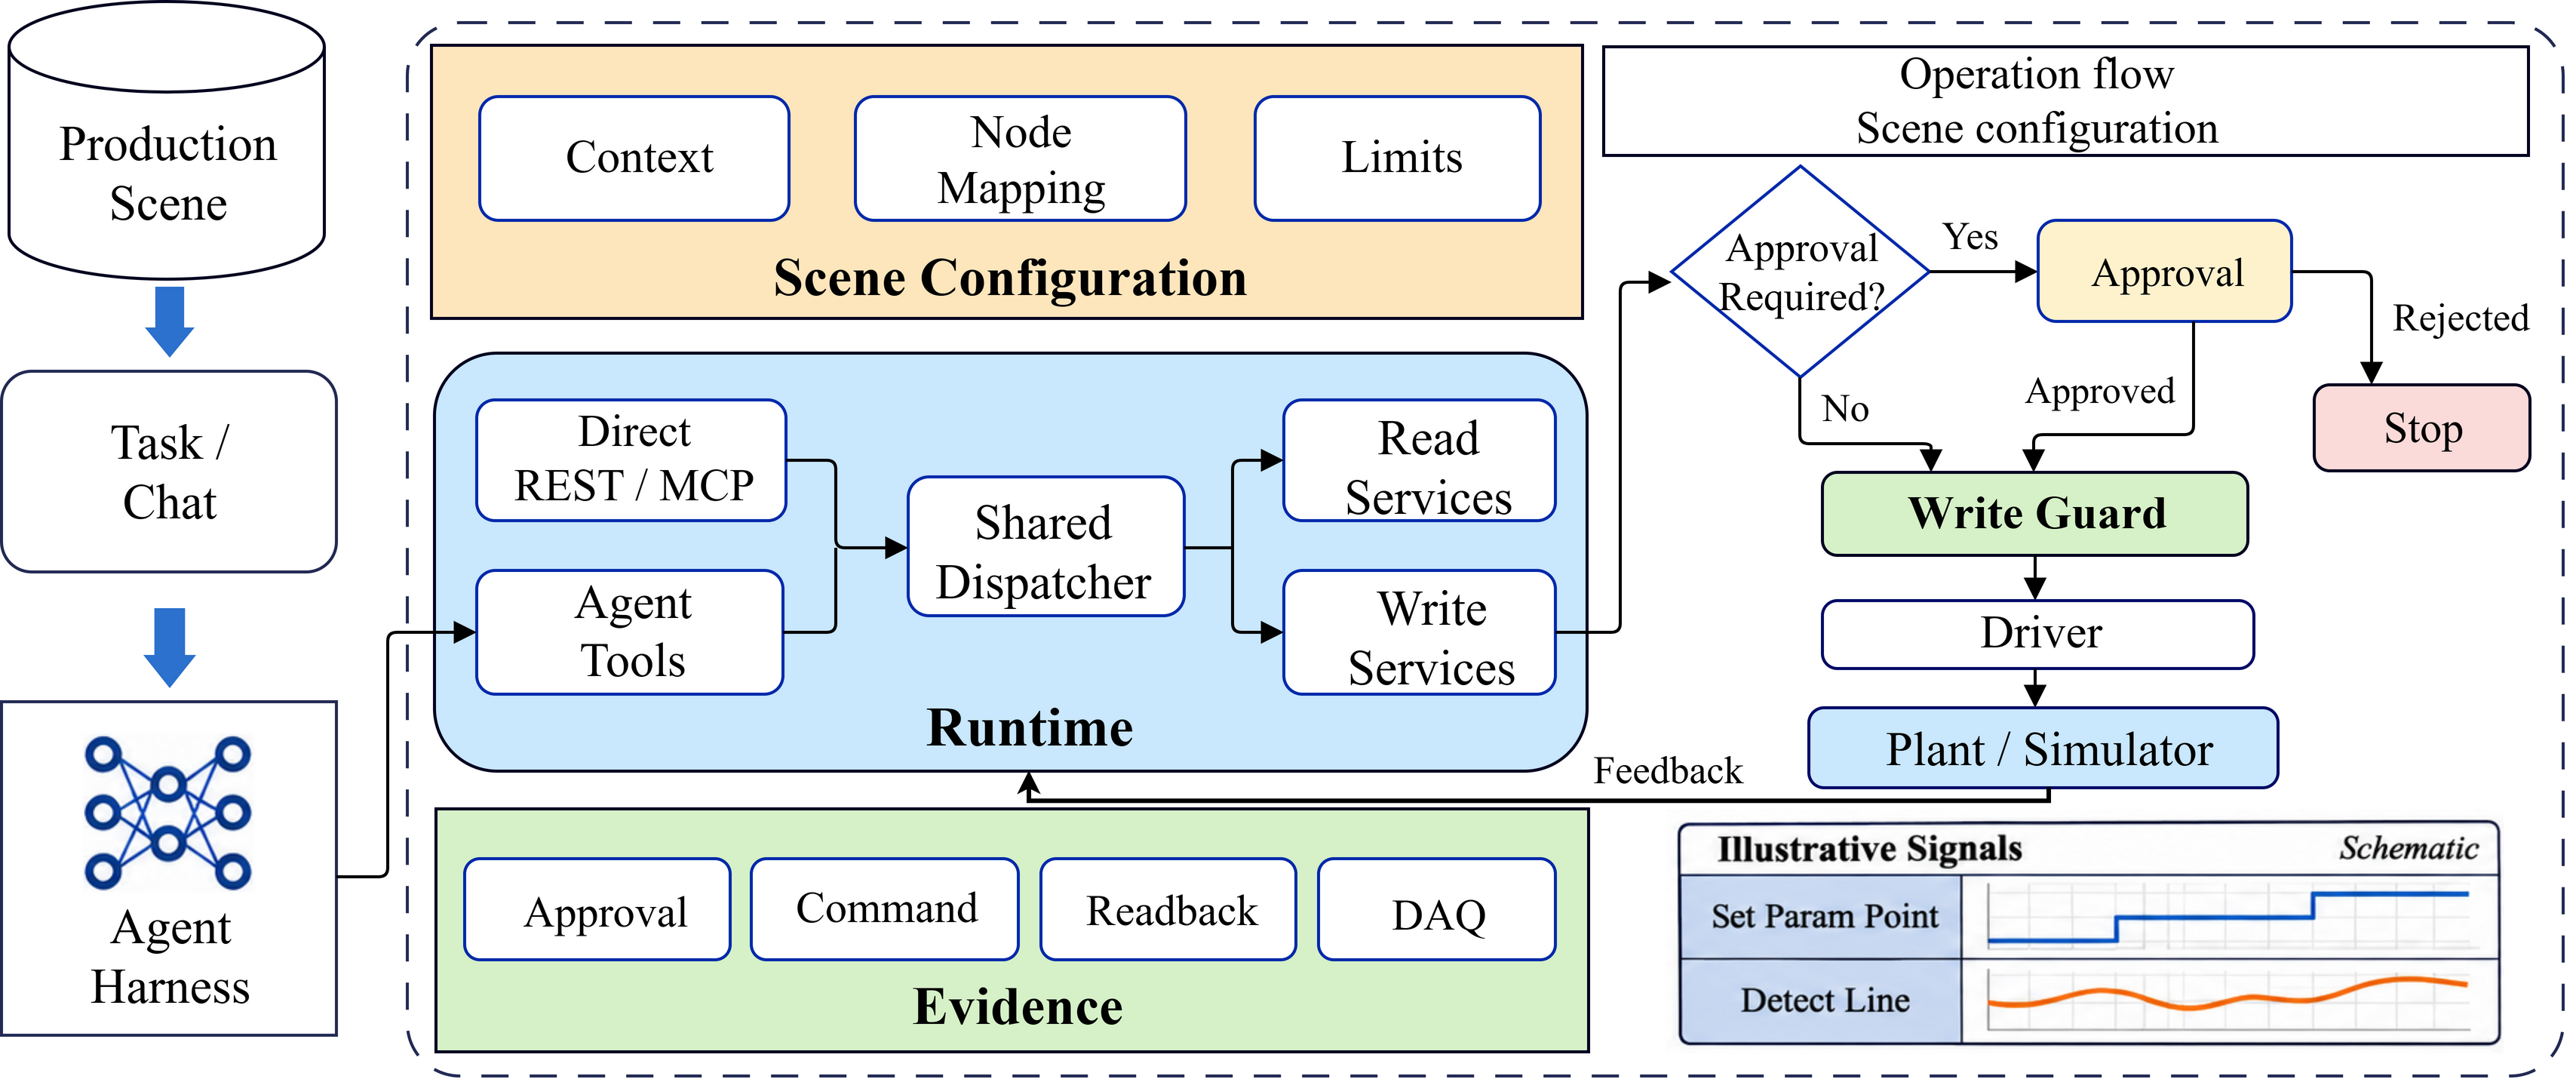
\includegraphics[width=\textwidth]{resources/fig2.png}
\caption{Task-mediated and direct tool calls share a dispatcher; a registered agent can acquire observations and submit a control intent, while direct calls provide a test entry point. Direct calls do not require a task. Approved intents undergo route-specific revalidation (omitted here; see Fig.~\ref{fig:hitl}). The no-approval path remains subject to applicable authorization and write guards. Requests rejected by pre-dispatch checks stop before driver dispatch. Feedback and signals are schematic, not measured traces. Approvals, command outcomes, optional readbacks, and later data-acquisition (DAQ) observations are distinct records. In-flight exclusion of overlapping writes per node and process is not shown; equipment interlocks remain necessary.}
\label{fig:arch}
\end{figure*}

\subsection{Design Rationale and Requirements}
\label{sec:principles}
The runtime must preserve process meaning across heterogeneous drivers, hold a stable contract for registered harness adapters, and check authority and process limits before every control write, keeping acquired process data, command acceptance, and later observations distinct. Scene configuration, registered adapters, shared dispatch, route handlers, and service-owned records enforce these boundaries.

For each agent turn, the context builder assembles the production context and eligible observations. The agent uses them to shape a proposal, but neither context nor observations grant write authority; the handler resolves live state when the operation is invoked.

\subsection{Layered Architecture}
\label{sec:layers}
Fig.~\ref{fig:arch} shows the layers: task and chat routes use registered harness adapters providing scoped acquisition and control tools, constrained by binding and by the policy of the agent's channel, its scoped execution context; agent analysis remains distinct from deterministic boundary checks, and the feedback path and signals are schematic.

Direct REST agent-tool calls and the stdio-MCP bridge bypass task execution and enter the shared dispatcher. The task route gives the agent context, acquisition targets, and objectives; operation services resolve control mappings and guards. Read and analysis services---DAQ, MES access, retrieval, and optional model services---are separated from write and recipe services. Input/output mappings connect semantic nodes to built-in or plugin drivers, and owning services retain task, command, observation, and configuration records.

\subsection{Scene Configuration as the Integration Boundary}
\label{sec:scene-config}
Scene-specific semantics are configured before use: the active line identifies the production context, product and recipe records supply applicable targets and limits, and the run record provides the current operating state. Semantic nodes bind process variables to direction-specific acquisition or control mappings, which the driver registry resolves to protocol implementations; \emph{semantic} here denotes a named process variable with a direction, unit, and configured mapping, not an OPC UA or Asset Administration Shell information model. Each agent-facing operation is named and typed, so a harness need not construct protocol-specific messages; a scene using a registered driver can supply different context and node mappings behind the same operation contract, while a protocol absent from the registry still requires a driver adapter.

In the cast-film preset, the MQTT command mapping \texttt{linespeed-sp} controls line speed in m/min, while the distinct \texttt{film-thickness} mapping reads thickness in $\mu$m; an agent can acquire the thickness observation, compare it with its objective, and propose a line-speed intent, which the runtime admits against the control node's limits. Sharing MQTT does not make either signal a substitute for the other.

Table~\ref{tab:scene-config} summarizes how the execution path uses the scene description, distinguishing configuration-time bindings from live-state checks. The context for an agent turn describes the active scene; before a write, the handler resolves the route's live state, applies current limits, and binds approval to both proposal and context where snapshots are supported (Section~\ref{sec:modules}). The command receipt remains separate from subsequent DAQ observations.

\begin{table*}[!t]
\centering
\caption{Scene configuration elements and their roles in the runtime path.}
\label{tab:scene-config}
\footnotesize
\setlength{\tabcolsep}{5pt}
\begin{tabularx}{\textwidth}{@{}>{\raggedright\arraybackslash}p{0.19\textwidth}>{\raggedright\arraybackslash}p{0.34\textwidth}X@{}}
\toprule
Element & Configured information & Runtime use\\
\midrule
Production context & Line, product, recipe, and run associations & Context construction for a task turn; route-dependent live-state checks before a write\\
Semantic I/O & Process variable, direction, unit, and node mapping & Acquisition uses the read mapping; accepted operations resolve the configured control mapping\\
Driver binding & Supported protocol driver and endpoint configuration & Driver registry selects the protocol implementation after operation checks\\
Operation admission & Engineering, baseline, product, and recipe limits; step and timing rules where configured & Route handler checks the candidate against current bounds and rejects inadmissible requests\\
Approval policy & Whether approval is required and the decision validity window & Pending request binds the proposed action; route-specific checks run after approval\\
Evidence ownership & Command receipt, verification grade, and later DAQ observations & Owning services retain command outcomes separately from process measurements\\
\bottomrule
\end{tabularx}
\end{table*}

\subsection{Cross-Module Execution Flow}
\label{sec:executionflow}
For a task-mediated call, the registered adapter presents a scoped tool
catalog containing acquisition, context, and control operations to the agent.
The agent reads available observations, relates them to the task objective, and
submits a typed intent rather than a protocol-specific message. At the
operation boundary, the shared dispatcher checks the predicates declared for
the named operation before selecting its handler. The handler resolves live
production state, applies route-specific guards and limits, and requests any
required approval before device I/O.

For an industrial operation $u$ by agent $a$ in channel $c$, the shared dispatch condition is
\begin{equation}
\mathcal{A}(a,c,u)=\bigwedge_{X\in\mathcal{C}(u)}X(a,c,u).
\label{eq:dispatch-contract}
\end{equation}
The dispatch predicates $S$, $P$, $G$, and $B$ in Eq.~(\ref{eq:dispatch-contract}) denote invocation scope, current channel policy,
the applicable industrial grant, and the agent's binding to referenced resources,
respectively. The declared set $\mathcal{C}(u)\subseteq\{S,P,G,B\}$ always contains
$S$ and $P$; the grant predicate $G$ joins when the resolved channel, target line, and owner/grant policy
require it, and the binding predicate $B$ joins when the operation declares resource references. Every included check must pass before handler
selection. Where configured, the policy predicate also covers channel tool
selection, profile, and duty-separation checks.

Once these predicates pass, the selected route applies its operational
guards and requests any required approval. For example, an exploration request checks
the control binding and DAQ visibility before entering the governed write
path; an invisible target returns an error before a write. The checks performed
after approval depend on the route; Section~\ref{sec:modules} specifies the
single-node and recipe-operation paths.

For a direct REST agent-tool call, the service establishes $a$ and $c$ before applying these checks: an agent token must match the requested agent identifier, an authenticated user must be the channel owner or an administrator, and the manager then loads the channel-agent record, rechecking scope and policy with any applicable grant and binding checks. Handlers resolve live production state
from request identifiers and the owning services.



\section{Agent-Coordinated Task-Level Operation}
\label{sec:closed-loop-operation}

\begin{figure*}[!t]
\centering
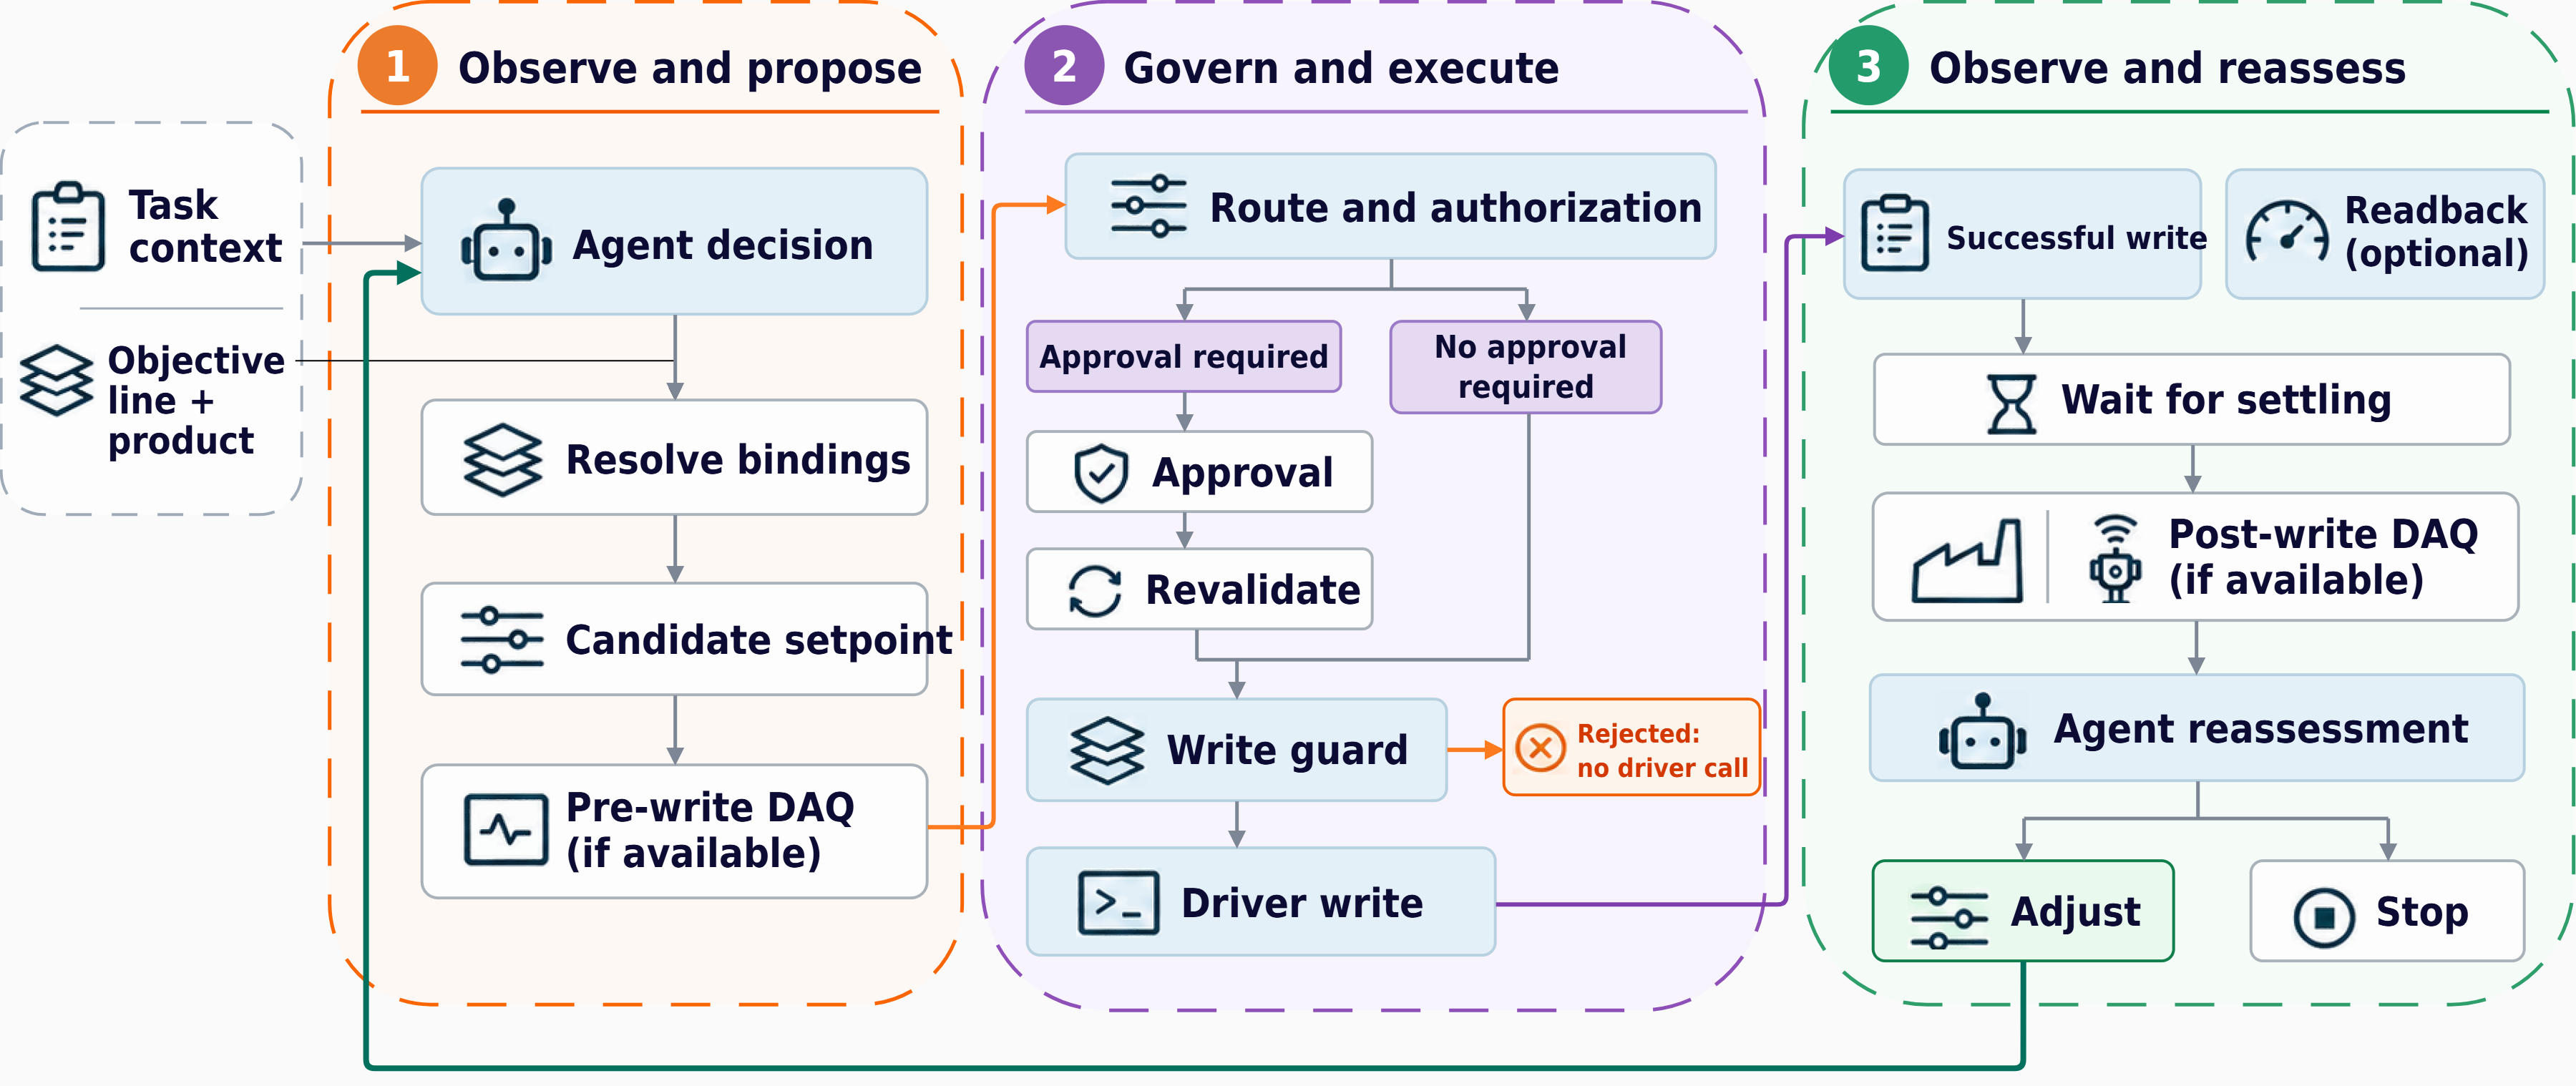
\includegraphics[width=\textwidth]{resources/fig3.png}
\caption{Intended task-mediated acquisition-to-reassessment flow, not a recorded run. The agent uses earlier observations (not shown); pre-write DAQ is an optional subsequent read. Route checks precede dispatch, and Fig.~\ref{fig:hitl} shows the omitted approval-denial path. ``Successful write'' in the diagram denotes reported command success, not verified actuation. A driver error may leave device state uncertain. Optional readback and later DAQ observations answer different questions: whether the setpoint matched and what the process subsequently did.}
\label{fig:agent-loop}
\end{figure*}

Fig.~\ref{fig:agent-loop} follows one intended task-mediated turn. Entry dispatch first establishes the caller, channel, and applicable policy; the route handler then resolves the operation's bindings and applies write-specific checks. The task supplies an objective and production context; the agent reads configured observations, assesses the gap to the objective, and proposes an adjustment. For single-node exploration, \texttt{optimization\_explore} resolves the control node from \texttt{control\_node\_id} or its binding, and resolves the DAQ target from an explicit ID or the agent's DAQ binding. In goal mode, a lead agent may decompose the objective and delegate this step as a worker subtask. The walkthrough is distinct from the scripted \texttt{recipe\_trial} contrast in Section~\ref{sec:eval-optimization}.

The operation resolves the applicable limit profile and control binding, then reads the stored value as $u_0$; this is not necessarily a fresh readback. The agent combines this state with its objective and direction. If direction is omitted, the operation defaults to an upward adjustment; otherwise $s\in\{-1,+1\}$. For a step $\Delta u$, it forms
\begin{equation}
 u^{*}=\operatorname{clip}\!\left(u_0+s\Delta u,\,u_{\min},\,u_{\max}\right).
 \label{eq:optimization-candidate}
\end{equation}
Clipping forms a proposal within configured tuning bounds (or node bounds if absent); it neither authorizes the write nor guarantees admission under Eq.~(\ref{eq:admission}). The effective step comes from the explicit argument, the binding's tuning step, the scene's maximum step, or one twentieth of the node range, in that order.

The operation resolves the DAQ target and checks visibility before the intent enters the governed path; gates added after the reported experiments (identifiability and model--ontology checks) are not exercised in Section~\ref{sec:eval}. If the checks pass, the operation attempts a pre-write DAQ read, whose mean may be unavailable.

A valid candidate enters the governed single-node write path in Algorithm~1: a pre-dispatch denial stops the request before any driver call, whereas a driver-stage error may occur after dispatch has begun, so status alone cannot establish whether the device changed and state must be reconciled before retrying.

After reported command success, the operation waits 10--300~s (45~s default) and attempts another DAQ read. It queries $[t_0-\tau,t_0]$ and $[t_0,t_1]$, with $\tau$ the pre-read window length and $t_1$ the later read time. The implementation sets $t_0$ before the pre-read and any approval wait, not at dispatch, so the second window can include pre-dispatch samples. Earlier code queried trailing 45-s windows instead. The means are descriptive, not causal estimates.

The exploration record stores the target, step, available DAQ means, and write status; the shared path separately records the command outcome and any available readback. The operation then returns an exploration summary. On a later turn, the agent can inspect the returned evidence, choose another step, or stop; iteration always requires a subsequent agent decision.



\section{Operation Governance and Evidence}
\label{sec:modules}
Section~\ref{sec:design} defined the shared dispatch contract. This section traces the agent's control intent from submission through scene-specific write admission,
conditional approval, and the records each route returns.

\subsection{Scene-Specific Write Admission}
\label{sec:governed}
Authorization and value admission are checked separately: the target band describes a desired process outcome, not the admissible write interval, and a candidate may satisfy all write constraints while the measured value remains outside the band.

For an online node write, the admissible value interval is
\begin{equation}
\mathcal{I}^{\mathrm{online}}_n(t)=
\mathcal{H}_n\cap\mathcal{L}^{\mathrm{base}}_n\cap\mathcal{L}^{\mathrm{prod}}_n(t)\cap\mathcal{L}^{\mathrm{rec}}_n(t),
\label{eq:admission}
\end{equation}
where $\mathcal{H}_n$ is the hard engineering range, and
$\mathcal{L}^{\mathrm{base}}_n$, $\mathcal{L}^{\mathrm{prod}}_n$, and
$\mathcal{L}^{\mathrm{rec}}_n$ are the baseline, active-product, and
active-recipe limits. These numerical bounds are distinct from the scope,
policy, grant, and binding predicates in Eq.~(\ref{eq:dispatch-contract}).
An absent optional limit imposes no restriction; an empty intersection admits no candidate, and the controller identifies the first violated layer when a limit is exceeded. Recipe dispatch checks a replacement recipe against the hard, baseline, and product limits rather than the previous recipe's window; trial overrides are additionally checked against the applicable recipe window.

Algorithm~1 details the single-node write sequence after shared dispatch; Fig.~\ref{fig:hitl} maps the same boundary across the single-node and recipe routes. For
\texttt{optimization\_explore}, the algorithm shows the ordinary full-limit profile: a failed
check stops the request before driver dispatch, while a benchmark ablation may
omit soft limits and retain the hard engineering range.

\par\medskip
\noindent\begin{minipage}{\columnwidth}
\small
\noindent\textbf{Algorithm 1:} Governed online single-node write
\par\kern2pt\hrule\kern2pt
\begin{algorithmic}[1]
\Require Node $n$, candidate $x$, and channel, if present
\Ensure Rejection or driver outcome and available readback
\State Check execution mode, value, and node authorization
\If{approval is required}
  \State Request a decision for $(n,x)$ and wait
  \If{decision is declined or expires}
    \State \Return rejection
  \EndIf
  \State Revalidate the original authorization path
\EndIf
\State Recheck the grant if a channel is present
\State Check gateway/node state and controller guards
\State Resolve $\mathcal{I}^{\mathrm{online}}_n$; reject if $x\notin\mathcal{I}^{\mathrm{online}}_n$
\If{not benchmark mode}
  \State Check step, interval, and hold window
\EndIf
\State Dispatch $x$ to the configured driver for $n$
\State \Return outcome and available readback
\end{algorithmic}
\kern2pt\hrule
\end{minipage}
\par\medskip

The operation accepts an agent control intent; recipe and rollback sources follow
their own paths. A driver-stage error may still leave device state uncertain. These
application-level checks complement equipment interlocks; they do not replace them.

\subsection{Approval, Execution, and Evidence}
\label{sec:mech}

\begin{figure}[t]
\centering
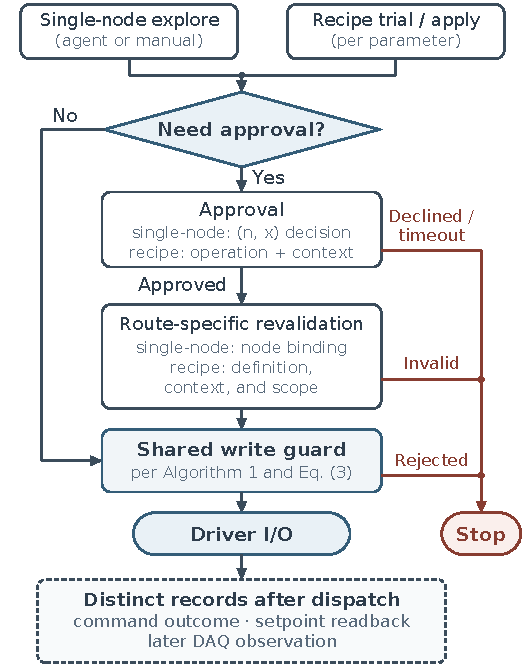
\includegraphics[width=\columnwidth]{resources/fig4-governed-flow.pdf}
\caption{Governed write routes. Both routes reach the write guard but select limits differently. Algorithm~1 and Eq.~(\ref{eq:admission}) describe the online single-node path, not recipe application. Skipping approval does not skip dispatch authorization or write checks. A failed pre-dispatch check stops the affected operation or parameter; recipe writes are not an atomic batch. Driver outcomes, optional readbacks, and later observations are distinct records.}
\label{fig:hitl}
\end{figure}
Fig.~\ref{fig:hitl} maps both write routes onto the shared write guard and the distinct records returned after dispatch; Algorithm~1 details the single-node check sequence. For a manual single-node \texttt{optimization\_explore} request, approval covers the node, proposed value, current effective interval, and rationale; the same boundary receives an agent's typed intent after acquisition and analysis. As in Algorithm~1, a decline or timeout stops the request. Approval triggers revalidation of the original direct node binding or, for recipes, the recipe binding and parameter membership. Single-node approval does not use the recipe-operation context snapshot described next. In either path, revalidation does not make the checks and the external device write atomic.

For \texttt{recipe\_trial} and \texttt{recipe\_apply}, approval is bound to the recipe operation and
active line--product--recipe--run context. After approval, the handler checks
authority and context again and verifies the recipe definition and
candidate scope before dispatch. A changed context, revoked binding, or
changed recipe definition prevents that proposal from proceeding. Recipe-trial approvals default to a 30-minute window; single-node approval waits expire after 180\,s. Outside benchmark mode, writes require a minimum 60-s interval after a setpoint change, and recipe trials a per-line cadence of 300~s.

A \texttt{recipe\_trial} submits a bounded batch from the agent's control intent through the configured driver and returns a result per parameter to the calling route. Parameters are attempted individually, so a batch can be partially applied; results and device state must be reconciled before any retry. A trial neither saves nor applies a recipe version; later DAQ observations can be retrieved separately before updating, applying, or rolling back the recipe.

As sketched in Fig.~\ref{fig:hitl}, receipts record the command outcome returned to the agent or caller, while observations record what followed in the process; results are graded readback-verified, transport-acknowledged, or unverified. For a successful recipe write not already readback-verified, the service may by default attempt up to three additional reads at 2\,s intervals where supported; recipe batches retain per-parameter verification outcomes. A readback-verified result means the returned value matched the request within the applicable tolerance; a transport acknowledgment alone does not establish that the device applied the value, and an unverified result does not establish a matching readback. DAQ stores later timestamped observations for the agent's next analysis turn, while recipe history, approvals, and task records remain with their owning services; identifiers and timestamps can link these records when available, but a later observation alone does not prove that the command caused the measured change.



\section{Experimental Evaluation}
\label{sec:eval}
The primary evidence comes from direct probes of configured write mappings and fixtures for selected guard and approval branches. A scripted simulator comparison, one injection-twin write, and three language-model episodes provide exploratory context. They do not establish parity between task and direct calls or a complete agent-to-device trace. The scripted comparison uses \texttt{recipe\_trial}, not the task-mediated \texttt{optimization\_explore} sequence in Section~\ref{sec:closed-loop-operation}.

Integrated checks used pre-existing platform and simulator services, generally in benchmark mode, which bypasses step, interval, and hold-window checks for agent or manual writes; ablations removed selected checks, and no cold-start deployment or physical-plant run was performed.

A service response, a simulated readback, and a later process measurement remain distinct throughout this section.

\subsection{Configured Mapping and Integration Checks}
\label{sec:eval-mapping}
Two integrated executions, both seed~42, each passed 77 assertions across 17 phases. Their tool-level loops were scripted; neither run used a language-model agent or constituted an independent deployment. A separate film-line preset check configured five endpoint types and rejected nine selected negative probes. These checks cover preset configuration and direct runtime/API behavior. The scene--protocol matrix below covers structural and value checks in the control direction, not validation of acquisition mappings; timing and hold-window checks are reported separately.

The scene--protocol probes covered 55 configured write-capable endpoints in four simulated scenes over five protocols: Modbus Transmission Control Protocol (TCP), Modbus remote terminal unit (RTU), OPC UA, MQTT, and Hypertext Transfer Protocol (HTTP). Table~\ref{tab:scene-probe-results} gives the scene-level counts. The probe plan specified three requests for interior values, one for the upper boundary, and four for values outside the structural range (the hard engineering range $\mathcal{H}_n$) at each endpoint. All 220 requests with prespecified admissible values received the expected acceptance response; all 219 collected structural-violation requests received the expected rejection, and all 216 available simulator readbacks matched the requested values. One nominal out-of-range candidate lay inside its endpoint's hard range and was filtered before dispatch, so the structural denominator is the 219 collected requests; the single HTTP endpoint provided no readback for its four admissible requests. Because the tested values, the guards, and the expected responses derive from the same configured limits, and the readbacks come from the same simulated stack, these counts show response consistency of the tested mappings, not independent verification. Not every protocol was tested in every scene, so the matrix characterizes selected mappings rather than general protocol interoperability.

\begin{table*}[!t]
\centering
\caption{Configured scene--protocol probes. Counts show prespecified admissible requests receiving the expected acceptance response, collected structural-violation requests receiving the expected rejection, and matching simulator readbacks where the endpoint supports them. The structural denominator is collected requests; one nominal candidate was filtered before dispatch.}
\label{tab:scene-probe-results}
\footnotesize
\setlength{\tabcolsep}{3pt}
\begin{tabularx}{\textwidth}{@{}>{\raggedright\arraybackslash}p{1.55cm}r X r r r@{}}
\toprule
Scene & Configured endpoints & Protocols represented & Accepted probes & Structural rejects & Simulator readbacks \\
\midrule
Injection & 11 & TCP 5; RTU 2; OPC UA 3; MQTT 1 & 44/44 & 44/44 & 44/44 \\
Wastewater & 7 & TCP 1; RTU 3; OPC UA 2; MQTT 1 & 28/28 & 28/28 & 28/28 \\
Annealing & 7 & TCP 3; RTU 2; OPC UA 1; MQTT 1 & 28/28 & 28/28 & 28/28 \\
Biaxial line & 30 & TCP 20; RTU 1; OPC UA 8; HTTP 1 & 120/120 & 119/119 & 116/116 \\
\bottomrule
\end{tabularx}
\end{table*}

\subsection{Exploratory Fixed-Horizon Simulator Contrast}
\label{sec:eval-optimization}
We compared a deterministic bounded setpoint policy with a no-write condition in injection, wastewater, and annealing simulations, using the \texttt{recipe\_trial} route. Candidate adjustments include injection holding pressure and time, wastewater blower and dosing settings, and annealing-zone temperatures and line speed, selected by scene-specific conditions. The target bands were $32.5\pm0.35$~g for part weight, $3.4\pm0.6$~mg/L for dissolved oxygen, and $95\pm6$~HV for hardness, respectively. Each scene used its own fixed horizon (180~s for injection; 240~s for the other scenes), nominal one-second sampling, an independent reset for each arm, and a pre-specified window for the initial process value. Arm order was randomized within each block; paired starts need not have identical process values. The primary outcome was integrated absolute error (IAE), the trapezoidal integral of the absolute deviation from the target-center value over the retained samples; it is not an integral to the nearest band boundary. Internal gaps up to 5~s were linearly interpolated; no extrapolation was made to the nominal window endpoints, and a larger gap invalidated the pair.

After a pilot batch, a later batch of 11 scene--seed blocks was collected; nine met the reset, initial-window, and sampling rules, and two (wastewater seed~45, annealing seed~46) were invalid through 9-s and 6-s no-write sampling gaps. An earlier batch contains a valid, independently reset injection seed-44 block ($\Delta\mathrm{IAE}=193.320$~g\,s; the later batch repeated it with 165.165~g\,s) and failed reset attempts; no batch-selection rule is documented, so the reported subset is exploratory. Every valid block in the later batch had a positive $\Delta\mathrm{IAE}=\mathrm{IAE}_{\mathrm{no\text{-}write}}-\mathrm{IAE}_{\mathrm{scripted}}$. Among valid blocks, every scripted run entered its target band; no no-write run did. Table~\ref{tab:selected-iae} reports per-scene medians and ranges for those nine blocks.

\begin{figure*}[!t]
\centering
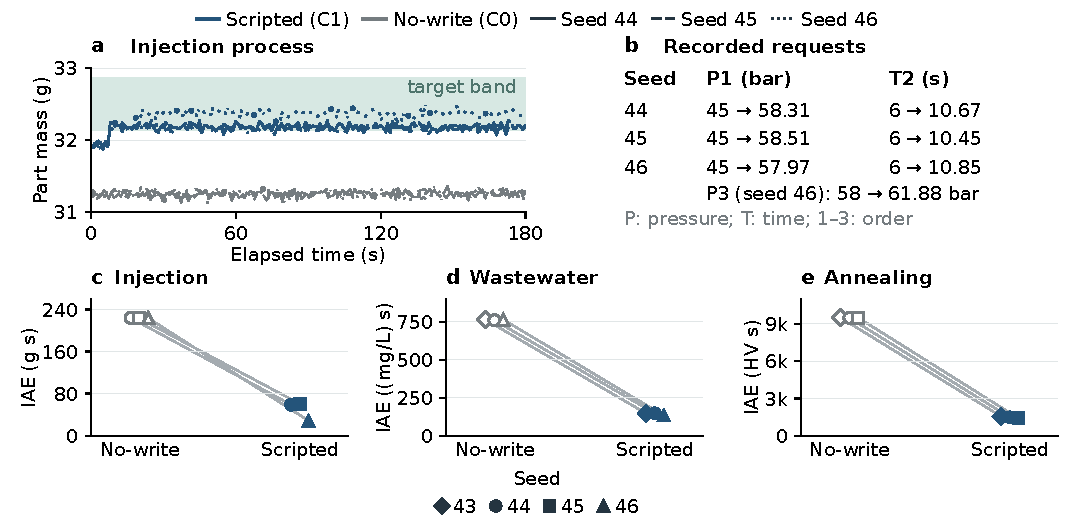
\includegraphics[width=\textwidth]{resources/fig5.pdf}
\caption{Selected exploratory simulator observations. (a) Recorded part-mass samples for the three valid injection scene--seed blocks over the nominal 180~s window; the shaded band is 32.15--32.85~g. Color distinguishes no-write (C0) from the scripted policy (C1), and line style identifies the seed. Sampling gaps beyond 1.5~s appear as breaks and isolated samples as dots; no smoothing is applied. (b) Recorded starting and requested setpoints: P and T denote hold pressure and hold time, and subscripts give request order, not timestamps. These are script records, not independent simulator-device readbacks. (c)--(e) Retained-window IAE for the nine selected scene--seed blocks; markers identify seeds. Each line connects one contrast, and small horizontal offsets only separate overlapping markers. Each scene uses its own scale and reports its native unit multiplied by seconds, so magnitudes are not comparable across scenes. The two blocks invalidated by sampling gaps and the earlier repeated injection block are excluded.}
\label{fig:optimization-trajectory}
\end{figure*}

\begin{table}[!t]
\centering
\caption{Exploratory fixed-horizon simulator contrasts; see text for selection and inference limits. IAE is integrated absolute error to the target-center value. Positive $\Delta$IAE means lower retained-window error under the scripted policy. The Valid column is valid/collected blocks in the later batch.}
\label{tab:selected-iae}
\footnotesize
\setlength{\tabcolsep}{3pt}
\begin{tabular}{@{}lcc@{}}
\toprule
Scene (unit of $\Delta$IAE) & Valid & Median (range) \\
\midrule
Injection (g\,s) & 3/3 & 165.165 (162.535--195.169) \\
Wastewater ((mg/L)\,s) & 3/4 & 615.605 (611.670--630.980) \\
Annealing (HV\,s) & 3/4 & 8000.450 (7930.200--8084.150) \\
\bottomrule
\end{tabular}
\end{table}

The run record's combined SHA-256 matches local copies of the paired-run and policy scripts, but does not identify the executed service image. Without complete service and simulator snapshots, the comparison cannot be reproduced end to end. No-write is a reference for describing the selected blocks, not a competing controller. We tested neither proportional--integral--derivative nor model-predictive control and make no claim about statistical significance, causal improvement, or comparative efficacy.

Fig.~\ref{fig:optimization-trajectory}(a) shows the mass traces of the three valid injection blocks, and (b) tabulates their recorded setpoint requests. Each scripted trace entered the band within 15~s and fluctuated near its lower boundary; no-write traces stayed near their initial values. The three task records report baseline part masses of 31.242, 31.2225, and 31.274~g, respectively; none is necessarily the first sample in the plotted horizon. Seeds~44 and~45 each recorded a pressure then a hold-time request; seed~46 added a further pressure request ($58\rightarrow61.88$~bar) after its hold-time request. The task script's final post-settling means were 32.163, 32.190, and 32.383~g, respectively, within the 32.15--32.85~g band. The starting and requested values in Fig.~\ref{fig:optimization-trajectory}(b) are script records, not independent device readbacks. For seed~46, a prior request to 57.97~bar precedes the later recorded starting value of 58~bar. The archive neither aligns requests with acquisition timestamps nor preserves a per-request server ledger. Fig.~\ref{fig:optimization-trajectory}(c)--(e) compare IAE for the nine selected blocks by scene; Table~\ref{tab:selected-iae} reports the contrasts.

\subsection{Write-Guard and Route Behavior}
\label{sec:eval-ablation}
The guard comparison used direct requests in one simulated scene with a mock driver. Four configurations retained or removed the process-window check (the configured recipe-window limit) and the readback check; Fig.~\ref{fig:guard-approval-results}(a) labels them full guard, no window, no readback, and neither. Hard structural limits stayed active. Each configuration ran three repetitions of four structural, two window, three legal, and three boundary inputs, excluding timed writes. All four rejected 12/12 structural violations and accepted 9/9 legal requests. Each configuration retaining the window check rejected 6/6 window violations (HTTP~400); each without it accepted 6/6 (HTTP~200). Each met its own 9/9 boundary expectations, which changed when the window check was removed. The inputs differed across configurations and the expectations came from the configured limits. This is evidence of the window branch's behavior, not a matched-input effect estimate. The repetitions do not constitute independent trials, HTTP responses do not establish driver dispatch, and this comparison produced no readback mismatch, so it does not assess the readback check.

In a separate follow-up batch, all 110 tested values---two per endpoint, outside the configured recipe window but within structural limits, across the same 55 endpoints---were rejected. In a readback-fault probe, a 230-unit command returned 251 and was graded \texttt{unverified} under a 0.7-unit tolerance; one baseline and one recovery call were \texttt{readback-verified}. Production-mode branch checks rejected one case each for interval, step, node range, recipe window, and hold window, and accepted a legal baseline; separate authorization checks rejected an unbound and a cross-node request and accepted a bound write. These fixtures characterize the selected branches and inputs, not physical-device safety.

The four approval-route calls used scripted decisions and did not follow the full task-mediated sequence; each invoked \texttt{optimization\_explore} directly. The approved call changed the simulated setpoint from 202 to 204.8; the rejected call left 216 unchanged. Two separate calls that bypassed approval changed 202 to 204.8 and 216 to 218.8. Fig.~\ref{fig:guard-approval-results}(b) shows these before and after values. The calls illustrate routing; they are neither a matched ablation nor a test of operator decisions. The route fixtures in this subsection did not exercise post-approval revalidation, approval expiry, \texttt{recipe\_apply} or rollback, in-flight exclusion, or the baseline and product limits of Eq.~(\ref{eq:admission}) in isolation.

\begin{figure*}[!t]
\centering
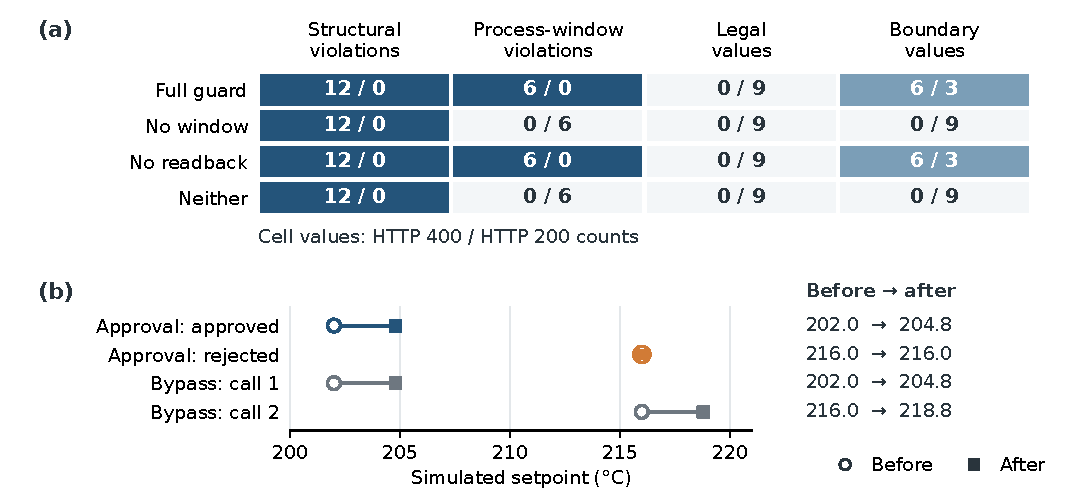
\includegraphics[width=\textwidth]{resources/fig6.pdf}
\caption{Guard-path comparison and scripted approval-route results. (a) Counts of HTTP~400 and HTTP~200 responses for four guard configurations and four request classes, with three repetitions per configuration. Each cell lists rejected/accepted counts, and their sum is the class total; shading represents the proportion of HTTP~400 responses. The specific violation values and boundary expectations differed across configurations. The comparison did not stimulate a readback mismatch. (b) Recorded before and after simulated setpoints for four separate calls; open circles mark before and filled squares after. A scripted proxy supplied the approval decisions, and the bypass calls required no approval. The calls are not matched pairs. HTTP~200 does not establish driver dispatch.}
\label{fig:guard-approval-results}
\end{figure*}

\subsection{Injection-Twin Demonstration}
\label{sec:eval-twin-pilot}
In one acceptance-script run on a PLC-based simulated twin (\texttt{realPlant=false}), a governed write changed holding pressure from 60 to 63.7~bar with matching simulated readback. Three later part-mass samples averaged 32.224~g. The structured and narrative baselines differ (31.503 and 31.508~g, respectively), and neither the raw series nor the complete runtime snapshot was retained. This run illustrates a write and readback, not a process effect.

\subsection{LLM-Driven Simulator Episodes}
\label{sec:eval-agent}
The \texttt{deepseek-flash} endpoint served three injection episodes. The saved worker label was blinded and the served model snapshot was not retained. All three episodes ended \texttt{CANCELED} below the 32.15--32.85~g band, at 31.70, 31.87, and 31.99~g. Each worker trace records one \texttt{recipe\_trial} call to update two setpoints and a response that acknowledged both; approval was automatic, and one episode was flagged for a guard violation. With no row-level server journal retained, these responses do not independently verify driver dispatch, and the episodes do not estimate agent success, approval effects, or physical execution.


\section{Discussion}
\label{sec:discussion}
The strongest evidence concerns the write boundary, not the agent's choice of a setpoint. Across the probed simulator mappings, admissible and inadmissible requests received their expected responses. In the mock-driver fixture, window violations were rejected in the two configurations that retained the window check and accepted in the two that did not, while structural violations were rejected in all four. This supports conformance on the tested branches, with expected responses based on the same configured limits. The endpoint matrix covers writes, not acquisition mappings or parity between task and direct calls.

The distinct records matter when interpreting the exploratory runs: a command outcome is not an independent dispatch record, a simulated readback is not physical actuation, and a later process measurement does not identify the effect of a write. The selected fixed-horizon comparison lacks a documented batch-selection rule and a controller baseline. None of the language-model episodes reached its target, and none retained a correlated acquisition-to-device trace. The runtime defines where an agent can propose and reassess an action; it does not demonstrate autonomous iteration.

A stronger evaluation would first retain a correlated task-mediated trace and compare both entry paths on the same cases, including read-direction checks and post-approval state changes. Process efficacy requires a prespecified study with verified resets, common sampling and horizons, complete trajectories, and a named controller baseline. Retained runtime and model snapshots would make agent trials auditable. Approval effects and physical safety require separate studies.

Two extensions remain future work: autonomous orchestration (a lead agent schedules governed steps and reassesses the results) and process-experience reuse (validated context, intents, and outcomes inform later proposals). Neither would confer write authority or bypass dispatch, approval, or revalidation.

\section{Conclusion}
\label{sec:conclusion}
We presented a configuration-driven runtime for connecting online observations and typed setpoint proposals to scene-specific mappings and governed execution. At 55 writable endpoints, all 220 prespecified admissible requests received the expected acceptance response, all 219 collected structural violations received the expected rejection, and all 216 available simulator readbacks matched. The mock-driver fixture rejected window violations only when the window check was enabled. These tests support conformance of selected write mappings and guards to their configured rules. The scripted comparison remains exploratory, and all three language-model episodes ended below the target band. Neither establishes complete agent-to-device execution, autonomous closed-loop control, comparative efficacy, or physical-plant safety. Separating command outcomes, readbacks, and later process observations makes clear what each record establishes. Autonomous orchestration and process-experience reuse remain future work within this boundary.


\section*{Acknowledgment}
The authors used generative AI via ZCode to edit the prose, draft the abstract, organize the LaTeX source, and lay out Fig.~\ref{fig:hitl}. The authors remain responsible for the manuscript.

\section*{Declarations}
The authors declare no competing interests. The study used simulated scenes, mock-driver fixtures, and a PLC-based simulated twin. It involved no human participants, personal data, or physical-plant data. Author contributions and funding are withheld during anonymous review. Selected simulator records and run summaries are available on reasonable request; complete service snapshots, raw twin samples, and row-level server journals were not retained.

\bibliographystyle{IEEEtran}
% \IEEEtriggeratref{10} removed 2026-11-13: with the longer data-availability
% statement the forced break spilled the remaining references onto an 11th
% page; natural flow ends on page 10.
\bibliography{resources/refs}

\end{document}

